\chapter{Interactive Video-on-Demand~System}
\label{chap:experiment}

\begin{figure}[t]
    \centering

    \subfloat[][System setup]{
        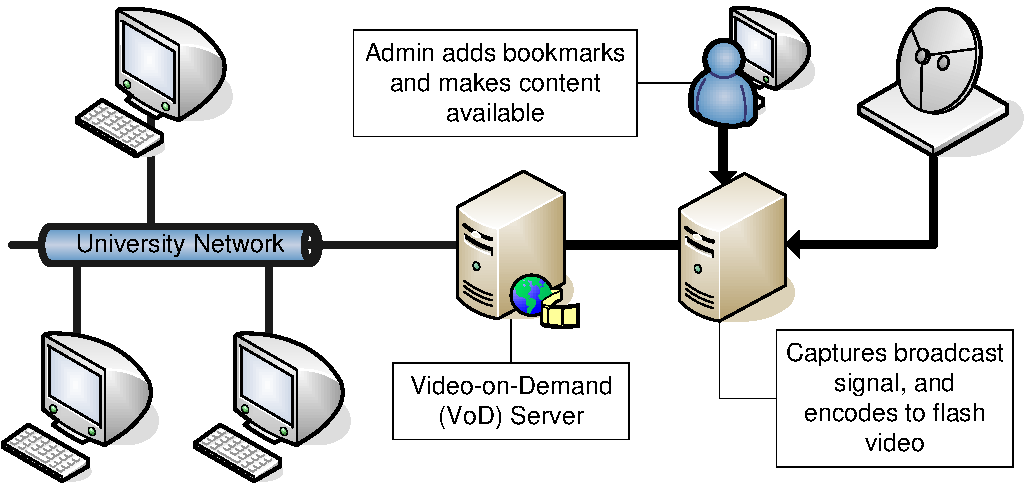
\includegraphics[width=0.5\columnwidth]{./diagrams/setup}
        \label{fig:system_setup}
    }
    \subfloat[][Player interface] {
        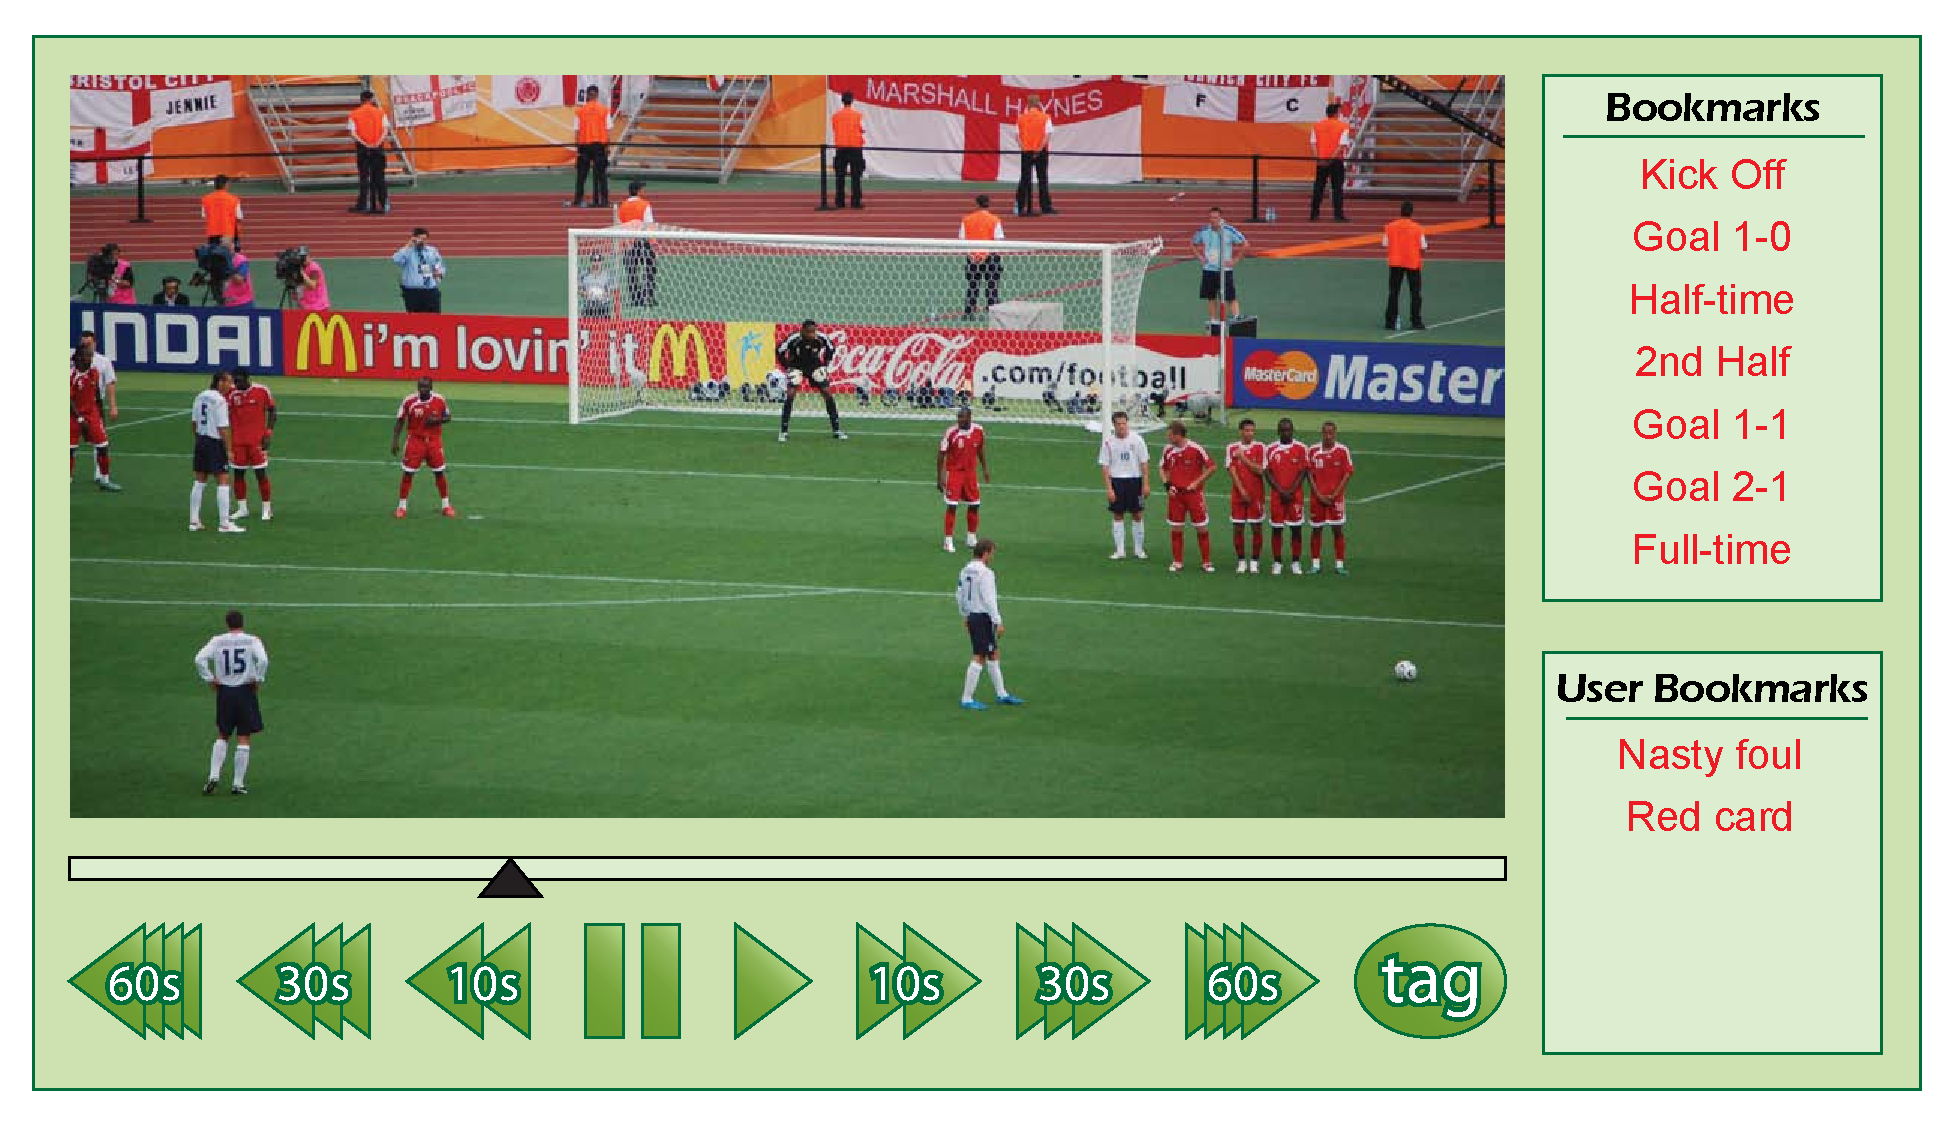
\includegraphics[width=0.5\columnwidth]{./diagrams/Interface}
        \label{fig:interface}
    }

    \caption{Diagrams of our video-on-demand system}
    \label{fig:system}
\end{figure}

There has been lots of work on characterising user behaviour when viewing video-on-demand (VoD) and streaming media (as discussed in \autoref{sect:characterisations}). However, there has been little analysis when a highly interactive system is used, for example, a system where users regularly pause and resume playback and actively seek around the media. This would generate results which would be a complete departure from the classic start-to-end model.

To obtain traces from a highly interactive workload, we set up and designed a video-on-demand system. This system was designed to provide powerful, yet simple interactivity controls, which would hopefully encourage more interaction between the users and the system. Once deployed, the system would be used to record traces of real user behaviour, and to be used as a test environment for future experiments. To be useful, the system had to meet three criteria:

\begin{description}
  \item[Wide user base] So that we could maximise the number of participants, the system needed to be designed in a way which was non-invasive, and simple for the users to use. This ruled out installing any special software on the users machines.

  \item[Encourage Interactivity] To ensure that the system generates a highly interactive workload, the layout of the user interface should make it easy to pause, resume, seek, \emph{etc.} This should be supported by the system, which should offer these features with low-latency, as to not to discourage their use.

      The content chosen for the system is also important. It should somehow encourage the use of interactive controls, for example, feature films will always be viewed start-to-finish, but genres such as sports may encourage users to view just the highlights.

  \item[Simple and Cheap] Finally, to ensure this system could be deployed, it has to be simple and cheap, for both us and the users. This of course can be achieved by using ``off the shelf'' products. Open source software would also be useful as it can easily be customised for our needs.

\end{description}

To meet all these requirements, the following choices were made. The system should be a simple client-server Flash based one, similar to the ones described in \autoref{sect:ugc}. These sites are relatively simple to set up and easily customisable. They also allow for a wide user base, as they use a simple web browser and the Flash player, both of which are commonly found on users' PC. These technologies will also typically work through firewalls, unlike other streaming protocols. This was beneficial to us, as it allowed us to stream to restricted users on our university campus.

The Flash player expects the video to be encoded as an FLV file; this can easily be achieved using the open source FFmpeg~\cite{ffmpeg}, which again makes this system simple and easy to deploy. One issue with the Flash player was the lack of seeking support, however a \emph{hack} was developed to add this functionality. The exact description of how this hack worked is described in \autoref{sect:seekable_flash}.

We chose a few different genres of content, but for the first round of experiments we served the 2006 FIFA World Cup. This is a hugely popular event with three to four matches on each day. Due to the number of matches each day, many users would miss the live match; this therefore encourages them to use our site to view any matches they missed.

The majority of videos served by our system typically had areas of particular interest, such as goals. To allow users to quickly navigate, we designed and added a \emph{bookmark} feature. While viewing the videos, the users were shown a list of bookmarks to the key events within the content. Then, at any point, the user could click the bookmark to instantly seek to its position within the media. Within our sport content, for example, goals, fouls and similar occurrences were bookmarked.

The concept of bookmarks in media is not new. Most DVDs contain chapter and scene bookmarks, which enable the user to start playback at any location. However, as far as we are aware, there have been no studies on how these DVD features are used. If a user does start a DVD at a specific chapter, it is no technical challenge for the DVD player to seek to the correct point and begin playback. This is not true for video-on-demand, as it can be quite strenuous for servers to seek arbitrarily. As such, the analysis of bookmark use within VoD will be novel.

The rest of this chapter explains how our video-on-demand system was designed and deployed to cater for our interactive experiments, and also outlines the different content used. This also includes the design of different tools to enable seeking within Flash videos.

\section{System Overview}

We set up a simple, interactive video-on-demand system. The system was divided into three main components: the capture server, the Video-on-Demand server, and a web interface as depicted in \autoref{fig:system_setup}.

% The capture server

Our capture server recorded publicly-broadcasted raw MPEG-2 streams of the programmes selected for our experiments. The recording was done via a digital TV capture device, using VLC~\cite{vlc} to store the raw stream. Once the full programme had been recorded, the system transcoded the stream with FFmpeg~\cite{ffmpeg}. Two streams were created; high and low bitrate Macromedia Flash 7 FLV files (1~Mbps and 300~Kbps respectively). Administrators would then manually add metadata to the system describing the files. This metadata included the title and description of the video as well as marking the location of key events within the videos which would become \emph{bookmarks} (more details on what was bookmarked is listed in \autoref{sect:experiment}). The final FLV files were then transferred to the VoD server, making them accessible to the users. The full procedure described typically took around twice the length of the recorded video, and so the videos were available shortly after being aired.

% VoD Server
The VoD system was an Apache webserver, which served the Flash-based user interface over HTTP. This server was only accessible to staff and students within Lancaster University's campus, and those staff and students connecting remotely via the university's Virtual Private Network (VPN). To aid in logging, all requests made through the user interface were verbose, allowing us to determine exactly which controls users pressed and when. Additionally, each playback window would maintain a periodic (10~second) HTTP-request heartbeat with the server, which was used to determine when connectivity was unexpectedly lost.

To handle user tracking, each user was assigned a unique session ID, which was stored within a HTTP cookie and their URLs. Each event that was logged contained this identifier, allowing us to track individual users throughout their visit to the site. If, however, a user blocked or deleted their cookie, they would appear to be new to the system upon each visit. We note within our analysis where this uncertainty could affect the results.

% Web interface
The web interface consisted of two main sections: an index page allowing the user to select any available video from the system, and the player interface that displayed the video (as shown in \autoref{fig:interface}). We were aware that the user interface would constrain the users' actions somewhat, and it was therefore designed to be as simple and generic as possible. We also wanted the interface to offer modern interactive controls (also called \emph{trick-modes}).

There are many different trick-modes, for example the ability fast-forward or rewind, or the ability to step through the video one frame at a time. However, offering too many trick-modes would clutter the interface, and most of them wouldn't be useful. Therefore, we limited the interface to having just seeking controls (\emph{e.g.} forward, backwards and to arbitrary points), as well as pausing and resuming.

Forward and backward buttons were provided that allowed seeking 10, 30 and 60 seconds in either direction. As these are relatively short distances, we also provided a \emph{seek bar} which enabled users to seek to any arbitrarily chosen time. Finally, a list of \emph{bookmarks} was displayed to the users, which enabled them to jump directly to key events. Bookmarks were added by an administrator, but later the interface was extended to also allow users to submit their own bookmarks (via the \emph{tag} button), which other users could see and use. User bookmarks often covered events that were not typically bookmarked, but were of particular interest (such as events that came under later scrutiny).
%
%\section{Logs}
%
%To analysis the behaviour of users of the system, numerous logs files were generated and later parsed. This section gives a brief overview of the log files, and how they were analysised.
%
%\begin{flushleft}
%\footnotesize
%
%[17-Jun 03:24:27] log.php?why=restart\&user=a044cb\ldots\&startBytes=0\&startTime=0\&seconds=0\&file=arg-scg\&action=seek
%
%[17-Jun 03:24:30] log.php?why=shortcut Goal 1-0\&user=a044cb\ldots\&startBytes=176378857\&startTime=1297\&seconds=1301\&file=arg-scg\&action=seek
%
%[17-Jun 03:24:37] log.php?user=a044cb\ldots\&seconds=1304\&file=arg-scg\&action=alive
%
%[17-Jun 03:24:47] log.php?user=a044cb\ldots\&seconds=1314\&file=arg-scg\&action=alive
%
%\ldots
%
%[17-Jun 03:30:57] log.php?why=back 30\&user=a044cb\ldots\&startBytes=913993735\&startTime=6719\&seconds=6720\&file=arg-scg\&action=seek~\\
%
%[17-Jun 03:30:58] log.php?why=back 60\&user=a044cb\ldots\&startBytes=905579160\&startTime=6659\&seconds=6660\&file=arg-scg\&action=seek~\\
%
%[17-Jun 03:30:59] log.php?user=a044cb\ldots\&seconds=6660.52\&file=arg-scg\&action=alive~\\
%\end{flushleft}

\section{Seekable HTTP Flash}
\label{sect:seekable_flash}

%\subsection{FLVTool++}
%\subsection{Seekable Flash}
% Flash is not seekable
%   When served from a website, it is streamed start-to-finish
%   Additional features needed to be added
%   Flash Indexing
%       Treat the file as a long continous series of frames
%       Playback can start from any keyframe
%       We create a index of keyframe file position
%       Thus to seek you resume playback from a specific position
%
%   Custom Player
%       To allow seeking a custom player needed to be designed
%       Designed using the standard Flash tools
%       Flash player could read FLV metadata
%       When a user seeked, the player found nearest keyframe
%       Player then issued request for the video + byte position
%
%   Server Side Support
%       The server must stream the video from offsets
%       Must do some magic to fix FLV headers
%

% Nic has read this

A few tools were created to enable a fully interactive experience in the experiments. Typically, when streaming Flash video (FLV) files from a web server, the full file is streamed start-to-finish, which does not allow for seeking to arbitrary points within the video. Therefore, additional software had to be developed to support seeking. This software was developed independently in 2006. However, in late 2007, YouTube implemented a system very similar to the one described here. The rest of this section discusses the three main changes which had to be implemented.

\subsection{Flash Indexing}

    It is not possible to start playback from any arbitrary byte within a media file, as a media player would have problems decoding the media. As such, an index is typically provided that maps byte offsets to seekable points within the media. The first application which was designed was one which could generate this index.

    Typically, stored video is contained within a single file as a long continuous sequence of frames. There is a frame for each picture within the video. Each frame has a unique timestamp, to represent the time at which it should be displayed, and typically these timestamps are at fixed intervals. In Flash video there are two types of frames; key frames and predictive frames. Key frames provide data to generate a full picture, whereas predictive frames provide only the differences since the previous key frame. This allows an efficient way to compress a video, where the complete picture typically does not change every frame.

    To play a video, the Flash player must always start at a key frame, otherwise a full picture can not be decoded. Thus, when seeking to an arbitrary point, the player must find the key frame immediately preceding the seek point. An index of key frames to positions within the file must be created to seek efficiently. This index can then be used to find the appropriate key frame when seeking.

    For our experiments, software was created to generate these indices. Each index was generated with a custom-made program named FLVTool++~\footnote{Since the release of this software, a product with the exact same name has been released by Facebook~\cite{flvtool}}. This C++ program scans through the FLV files, noting the byte offset of each key frame. Once all key frames were found, an index of the timestamps to byte positions was inserted into the beginning of the FLV file as meta data.

\subsection{Custom Video Player}
%       To allow seeking a custom player needed to be designed
%       Designed using the standard Flash tools
%       Flash player could read FLV metadata
%       When a user seeked, the player found nearest keyframe
%       Player then issued request for the video + byte position

    Once a FLV file has a key frame index, the Flash video player must be modified to take advantage of this. The Flash player provides a set of APIs which allows simple control over the playback of video. However, it does not provide any control for seeking. Therefore, to provide the appearance of seeking, each time a seek request was issued the Flash player would request a new video stream from the server. This requested video stream URL was in the form of:

    \begin{center}
    http://\bracket{host}/play.php?video=\bracket{video name}\&offset=\bracket{offset}
    \end{center}

    This URL allowed the server to start streaming from a specified offset, and thus the user could seek arbitrarily. The offset sent to the server is the byte offset for the requested key frame within the video file. This position is calculated by the Flash video player using the key frame index contained within the stream's meta data.

    Using the URL to pass the offset is not the best way to achieve this. The HTTP/1.1 standard has a \emph{Range} header~\cite{rfc2616}, which allows HTTP clients to partially request segments of files stored on a HTTP server. The better way to achieve seeking with Flash would be via this Range header, however the Flash player does not support this functionality. If it did, it would simplify processing on the server and aid in caching of the media by traditional web caches.

\subsection{Server Side Support}
    %Nic has read this

    As each seek is actually a new HTTP request for a stream starting at a specific offset, there must be some logic on the server which allows the client to begin from any offset within the stream. To achieve this, a PHP script was created which simply opened the file and streamed from the desired offset. This offset was provided in the URL by the client, who found the particular offset using the media's key frame index.

    Since the offset points to the beginning of a key frame, an FLV stream header is not present. Since each seek is a new stream, the header is required, as it contains information required for correct playback. Therefore, the PHP script recreates the correct header, and prefixed it to the stream.

    Because the video is served as a normal HTTP request, the server will try and transmit the stream as fast as possible. To conserve bandwidth and increase the maximum number of concurrent users, the server was configured to limit the streaming rate. For the first few seconds, the rate was unlimited and then afterwards limited to the video's average bitrate. This minimised the start-up latency and then smoothed playback afterwards.

%\subsection{P2P Simulator}

\section{Experiment}
\label{sect:experiment}
    Over the course of twelve months, this interactive video-on-demand system was used to carry out multiple experiments. These experiments were available to staff and students, and publicised to help attract users. The experiments were run in two phases, firstly covering the 2006 FIFA World Cup\footnote{This is not the only study to look at the 2006 FIFA World Cup, Silverston and Fourmaux took measurements of the PPLive peer-to-peer network as it broadcasted live matches from the event~\cite{silverston2007mpi}.} and nine months later a wider range of sport and musical events. The content selections were chosen because they had points of interest to bookmark, and would yield sufficient user demand.

    The first experiment made a total of 66 matches available from the World Cup (64 from the event itself, and 2 pre-competition friendlies) starting from the 9\sth of June 2006. Only results after the 13\sth of June were analysed due to alterations made to the logging system and user interface before that date. Each match was recorded from the beginning of the pre-match commentary through to the end of coverage. At the very least, every goal, penalty, and match start/end-point (inclusive of half-time) was bookmarked.

    As a direct result of the first experiments, some new autonomic management techniques were designed. To test this in a real environment, a second experiment was set up. From the 13\sth of April 2007, we began adding new content to extend the existing catalogue of content. This time, our approach was designed to test the various new techniques and to revalidate our previous experimental results. Furthermore, we wished to determine the relevance of our analysis/models to other genres (such as music).

    Over the following two months we provided the last six matches from the 2007 UEFA Champions League football tournament, some other miscellaneous football matches, seven Formula~1 races, as well as several recordings from music channels and the 2007 Eurovision Song Contest semi-final and final. The football matches were bookmarked in the same manner as the previous World Cup event. In the Formula~1 content we bookmarked the beginning and end of the race, as well as any noteworthy events such as a driver having to retire (after a crash or technical difficulties). Within the musical content the beginning of each track was bookmarked with its corresponding artist and title. A similar approach was taken with the Eurovision Song Contest, where the beginning of each song was bookmarked with the name of the country taking part.

    In total there were 88~videos, with an average length of 2.5~hours. The maximum video length was 4~hours, and the minimum length 45~minutes. There were 695~bookmarks, with each video having on average 7.8. 